% id: 30-22
% book: 베이직쎈 확률과 통계 · 02 중복조합과 이항정리
% section: 개념 09 파스칼의 삼각형
% figure: tikz:fig-30-22
% answer: 
% answer_source: 
% variant_level: 0 (원본 전사)
% 이 파일은 build.mjs 가 items.json 에서 만든다. 고칠 때는 items.json 을 고친다.
\smash{\raisebox{1.5mm}{\dmkichul{베이직쎈 확률과 통계 30쪽 22번}}}
\noindent\begin{minipage}[t]{0.58\linewidth}\vspace{0pt}\raggedright 오른쪽 파스칼의 삼각형에서 $\square$ 안에 알맞은 수를 써넣고, 파스칼의 삼각형을 이용하여 다항식 $(x+y)^5$을 전개하시오.\end{minipage}\hfill\begin{minipage}[t]{0.4\linewidth}\vspace{0pt}\centering \resizebox{\ifdim\width>\linewidth\linewidth\else\width\fi}{!}{% 30-22(인쇄 30쪽) — 빈 네모(□)가 섞인 파스칼의 삼각형 5단계까지. 스캔 화질이 낮아 TikZ 로 다시 그림.
% 원문에 찍힌 수(1, 2, 3, 4, 5)만 적고 □ 는 빈 네모로 둔다 — 답이 그림에서 읽히지 않게.
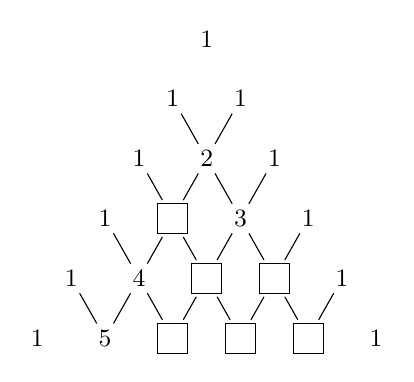
\begin{tikzpicture}[line width=0.4pt, font=\small,
  num/.style={inner sep=1.2pt},
  bx/.style={draw, line width=0.4pt, minimum size=3.8mm, inner sep=0pt},
  link/.style={line width=0.4pt, shorten >=1.2pt, shorten <=1.2pt}]
  % 행 k · 왼쪽부터 i 번째: x=(i-k/2)*0.86, y=-0.76k
  \node[num] (a00) at (0,0) {$1$};
  \node[num] (a10) at (-0.43,-0.76) {$1$};
  \node[num] (a11) at (0.43,-0.76) {$1$};
  \node[num] (a20) at (-0.86,-1.52) {$1$};
  \node[num] (a21) at (0,-1.52) {$2$};
  \node[num] (a22) at (0.86,-1.52) {$1$};
  \node[num] (a30) at (-1.29,-2.28) {$1$};
  \node[bx]  (a31) at (-0.43,-2.28) {};
  \node[num] (a32) at (0.43,-2.28) {$3$};
  \node[num] (a33) at (1.29,-2.28) {$1$};
  \node[num] (a40) at (-1.72,-3.04) {$1$};
  \node[num] (a41) at (-0.86,-3.04) {$4$};
  \node[bx]  (a42) at (0,-3.04) {};
  \node[bx]  (a43) at (0.86,-3.04) {};
  \node[num] (a44) at (1.72,-3.04) {$1$};
  \node[num] (a50) at (-2.15,-3.80) {$1$};
  \node[num] (a51) at (-1.29,-3.80) {$5$};
  \node[bx]  (a52) at (-0.43,-3.80) {};
  \node[bx]  (a53) at (0.43,-3.80) {};
  \node[bx]  (a54) at (1.29,-3.80) {};
  \node[num] (a55) at (2.15,-3.80) {$1$};
  % 이웃하는 두 수를 아래 수에 잇는 짧은 선(가장자리 1 에는 선이 없다 — 원문대로)
  \draw[link] (a10) -- (a21); \draw[link] (a11) -- (a21);
  \draw[link] (a20) -- (a31); \draw[link] (a21) -- (a31);
  \draw[link] (a21) -- (a32); \draw[link] (a22) -- (a32);
  \draw[link] (a30) -- (a41); \draw[link] (a31) -- (a41);
  \draw[link] (a31) -- (a42); \draw[link] (a32) -- (a42);
  \draw[link] (a32) -- (a43); \draw[link] (a33) -- (a43);
  \draw[link] (a40) -- (a51); \draw[link] (a41) -- (a51);
  \draw[link] (a41) -- (a52); \draw[link] (a42) -- (a52);
  \draw[link] (a42) -- (a53); \draw[link] (a43) -- (a53);
  \draw[link] (a43) -- (a54); \draw[link] (a44) -- (a54);
\end{tikzpicture}
}\end{minipage}\par
